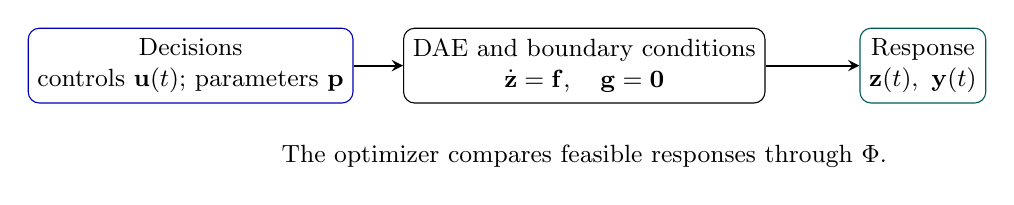
\begin{tikzpicture}[>=stealth,box/.style={draw,rounded corners,align=center,font=\small,minimum height=.95cm}]
\node[box,draw=blue!70!black](d)at(0,0){Decisions\\controls $\mathbf u(t)$; parameters $\mathbf p$};
\node[box](m)at(5,0){DAE and boundary conditions\\$\dot{\mathbf z}=\mathbf f,\quad\mathbf g=\mathbf0$};
\node[box,draw=teal!70!black](s)at(9.3,0){Response\\$\mathbf z(t),\ \mathbf y(t)$};
\draw[->,thick](d)--(m);\draw[->,thick](m)--(s);
\node[font=\small]at(5,-1.15){The optimizer compares feasible responses through $\Phi$.};
\end{tikzpicture}
